\chapter{Ausarbeitung}
\section{a}
Für einen Punkt gibt es:
\begin{equation*}
	\begin{bmatrix}
		v_E \\
		v_N
	\end{bmatrix} = \begin{bmatrix}
		0 & -\omega_3 & \omega_2 \\
		\omega_3 & 0 & -\omega_1 
\end{bmatrix} \begin{bmatrix}
	x \\
	y \\
	z
\end{bmatrix} = \begin{bmatrix}
	0 & z & -y \\
	-z & 0 & x 
\end{bmatrix} \begin{bmatrix}
	\omega_1 \\
	\omega_2 \\
	\omega_3
\end{bmatrix}
\end{equation*}
$v_E$ und $v_N$ sind die Geschwindigkeit in ENU System jeweils in Ost und Nord Richtungen und können wie folgt berechnet werden:
\begin{equation*}
	\begin{bmatrix}
		v_E \\
		v_N
	\end{bmatrix} = (\bm{R}_3(-\frac{\pi}{2} - \lambda) \cdot \bm{R}_1(-\frac{\pi}{2} - \phi))^{-1} \cdot \begin{bmatrix}
	v_x \\
	v_y \\
	v_z
\end{bmatrix}
\end{equation*}
wobei $\lambda$ und $\phi$ die Länge und Breite sind.\\\\
Dann kann man die Ausgleichungsmodell aufstellen. 
\begin{equation*}
	\bm{Y} = \bm{A} \cdot \bm{x}
\end{equation*}
wobei:
\begin{gather*}
	\bm{Y} = \begin{bmatrix}
		\bm{v_E} \\
		\bm{v_N}
	\end{bmatrix} \\
	\bm{A} = \begin{bmatrix}
		\bm{0} & \bm{z} & -\bm{y} \\
		-\bm{z} & \bm{0} & \bm{x} 
	\end{bmatrix} \\
	\bm{x} =  \begin{bmatrix}
		\omega_1 \\
		\omega_2 \\
		\omega_3
	\end{bmatrix}
\end{gather*}
Um die LSC durchzuführen, ist eine Kovarianz Funktion notwendig, diese Funktion definiert man wie folgt:
\begin{equation*}
	K(d) = \frac{K_0}{1 + (\frac{d}{a})^2}
\end{equation*}
$K_0 = 1.36\ut{mm^2/year^2}$, $a = 150 \ut{km}$ und $d$ die Abstand der 2 Punkten. Damit kann man $\bm{Q}_{ss}$,  $\bm{Q}_{s's'}$ und $\bm{Q}_{sy}$ bestimmen weil die Koordinaten bekannt sind. \\\\
Dann berechnet man $\bm{x}$ und die interpolierte Geschwindigkeit:
\begin{equation*}
	\bm{Q}_{yy} = \bm{Q}_{s's'} + \bm{Q}_{ee}
\end{equation*}
\begin{equation*}
	\bm{\hat{x}} = (\bm{A'}\bm{Q}_{yy}\bm{A})^{-1}\bm{A'}\bm{Y} = \begin{bmatrix}
		-2.98 \cdot 10^{-9} \\
		3.87 \cdot 10^{-9} \\
		-2.26 \cdot 10^{-11}
	\end{bmatrix} \ut{rad/year}
\end{equation*} 
\begin{equation*}
	\bm{\hat{s}} = \bm{Q}_{sy} (\bm{Q}_{yy})^{-1} (\bm{Y} - \bm{A}\bm{\hat{x}})
\end{equation*}
\begin{equation*}
	\bm{A}_{inter} = \begin{bmatrix}
		\bm{0} & \bm{z}_{inter} & -\bm{y}_{inter} \\
		-\bm{z}_{inter} & \bm{0} & \bm{x}_{inter} 
	\end{bmatrix} 
\end{equation*}
\begin{equation*}
	\bm{Y}_{inter} = \bm{A}_{inter} \cdot \bm{\hat{x}} + \bm{\hat{s}}
\end{equation*}
Die Geschwindigkeit Karte liegt in \autoref{fig:vel} und die Residuan in \autoref{fig:resivel}. Wegen falsche Skalierung der Matlab Funktion 'quiverm', werden Field 2 mal gezeichnet, wo einmal mit richtige, Skalar.
\begin{figure}[htpb]\centering
	\subfigure[]{
		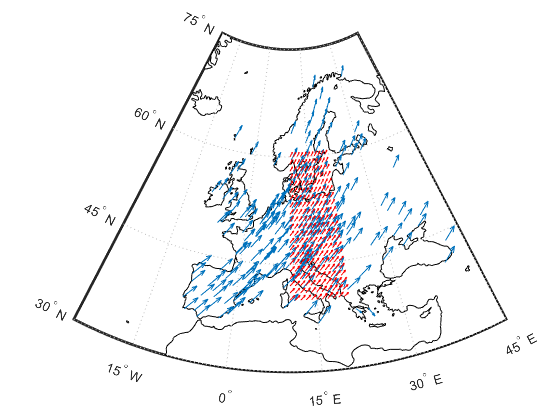
\includegraphics[width=0.9\textwidth]{velField1.png}}
	\subfigure[]{
		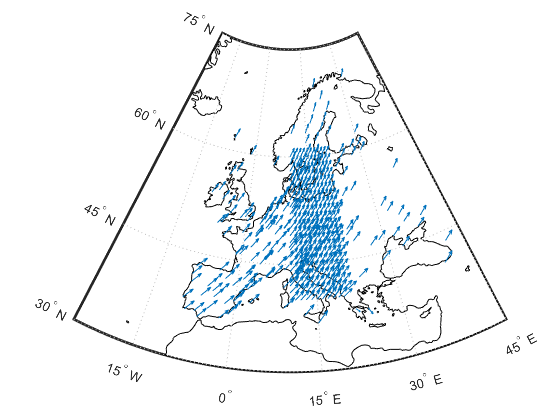
\includegraphics[width=0.9\textwidth]{velField2.png}}
	\caption{Geschwindigkeit}
	\label{fig:vel}
\end{figure}
\begin{figure}[htpb]\centering
	\subfigure[]{
		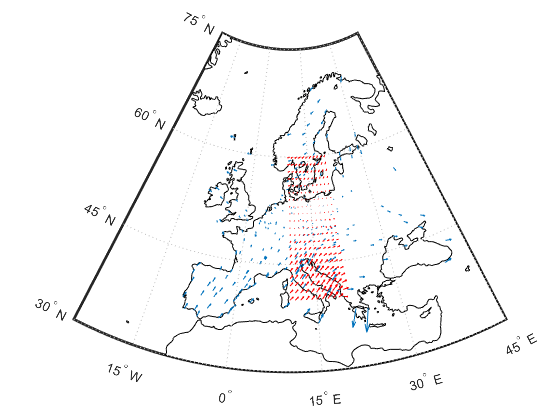
\includegraphics[width=0.9\textwidth]{resivelField1.png}}
	\subfigure[]{
		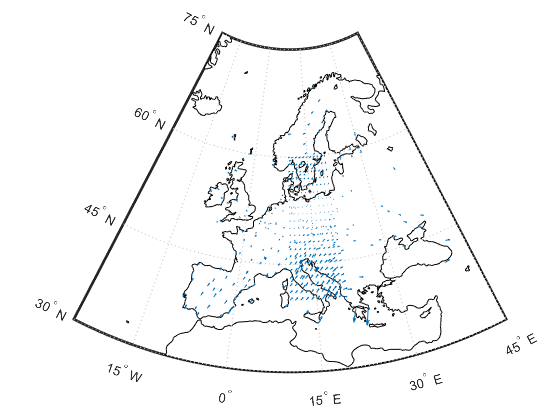
\includegraphics[width=0.9\textwidth]{resivelField2.png}}
	\caption{Resifual Geschwindigkeit}
	\label{fig:resivel}
\end{figure}\\\\
Die Varianz-Kovarianz werden auch berechnet:
\begin{gather*}
	\bm{H} = \bm{Q}_{sy} (\bm{Q}_{yy}) \\
	\bm{G} = (\bm{A'} \bm{Q}_{yy}^{-1} \bm{A})^{-1} \bm{A'} \bm{Q}_{yy}^{-1} \\
	\bm{Q}_{\bm{\hat{x}}} = (\bm{A'} \bm{Q}_{yy}^{-1} \bm{A})^{-1}  = \begin{bmatrix}
		9.27 & 1.80 & 9.88 \\
		1.80 & 2.22 & 2.37 \\
		9.88 & 2.37 & 13.04
	\end{bmatrix} \cdot 10^{-15} \\
\end{gather*}
